\section{Ap\'endice: Framework de Benchmarking} \label{casos_de_prueba}
\subsection{Descripcion de los metodos de benchmarking utilizados y presentacion de graficos}
\subsection{Resultados}
\subsubsection{Algoritmo exacto para la resolucion de CACM}
\subsubsection{Heur\'istica golosa}

En la experimentaci\'on de perfomance de la heur\'istica golosa utilizamos un generador de grafos aleatorios, hacemos variar la cantidad de nodos, con una cantidad de aristas fija. Sea $n$ la cantidad de nodos, es nuestra variable y probamos con $m = (n^2)/2$, es decir grafos completos, y luego con grafos densamente promedio, un n\'umero de aristas promedio entre $n-1$ (\'arbos) y un grafo completo ($ m = (n - 1 + (n^2)/2) /2 $)

\begin{center}
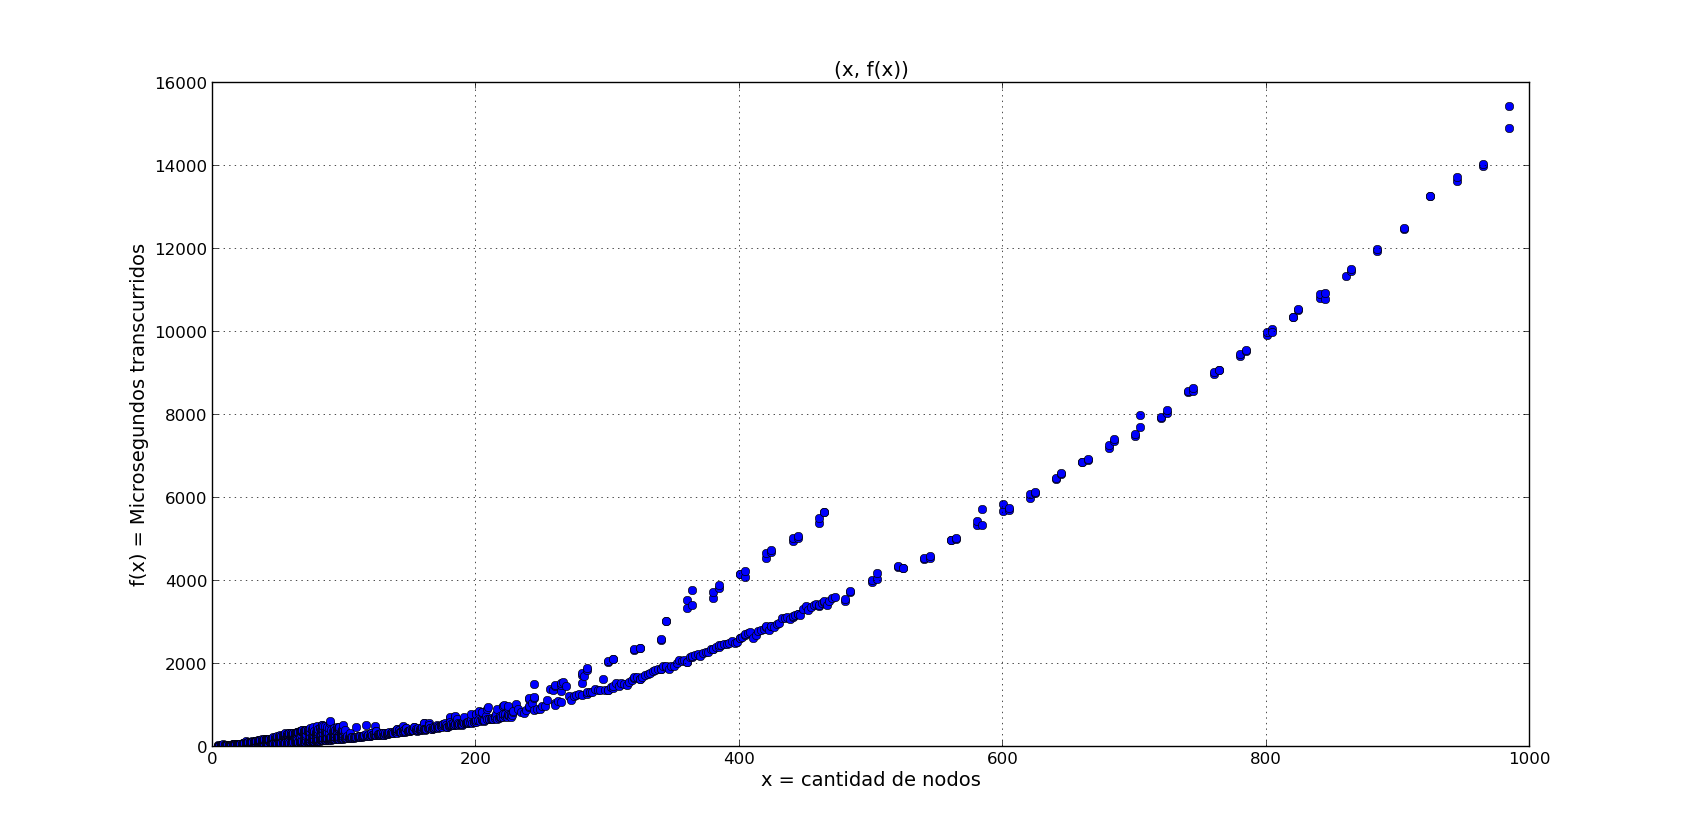
\includegraphics[scale=0.40]{img/golosa_fx.png}
\end{center}
\vspace{2mm}

Se puede apreciar una curva creciente con concavidad positiva. Vamos a dividir los resultados por $n^2$ y verificar que el resultado sea una curva constante.


\begin{center}
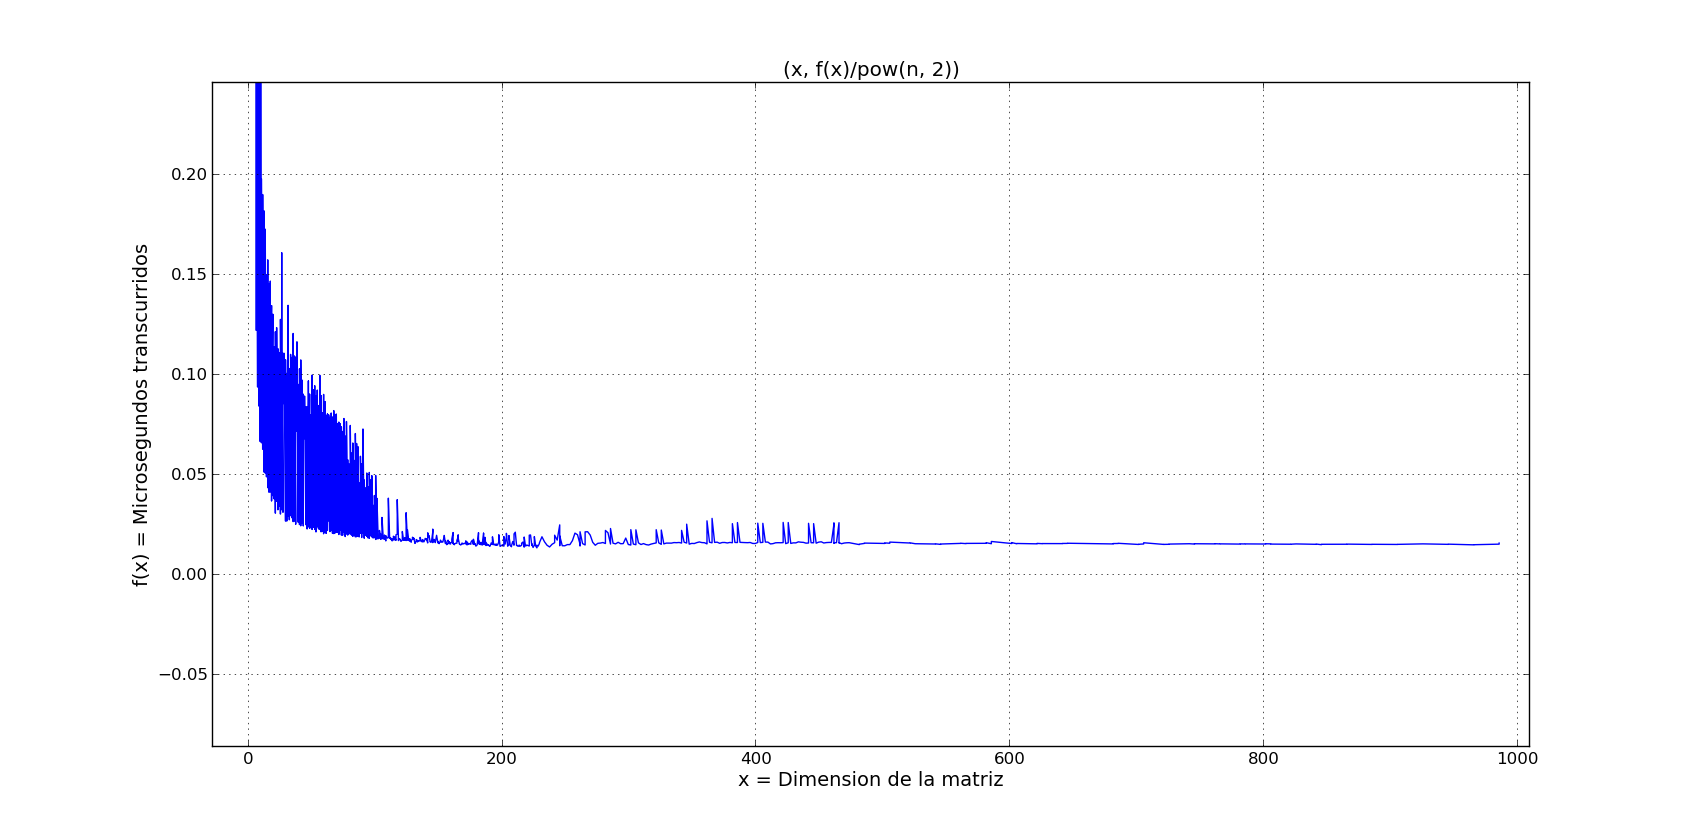
\includegraphics[scale=0.40]{img/golosa_fx2.png}
\end{center}
\vspace{2mm}

\subsubsection{Heuristicas de busqueda local}
\subsubsection{Metaheuristica GRASP: Solucion propuesta}
